%%==========================================================================%%
%% Author : Sa�udo Olmedo, Ignacio                                          %%
%% Author : S�nchez Barreiro, Pablo                                         %%
%% Version: 1.2, 21/04/2014                                                 %%
%%                                                                          %%
%% Memoria del Proyecto Fin de Carrera                                      %%
%% M2M/Caso de estudio                                                      %%
%%==========================================================================%%

\begin{figure}[!tb]
  \centering
  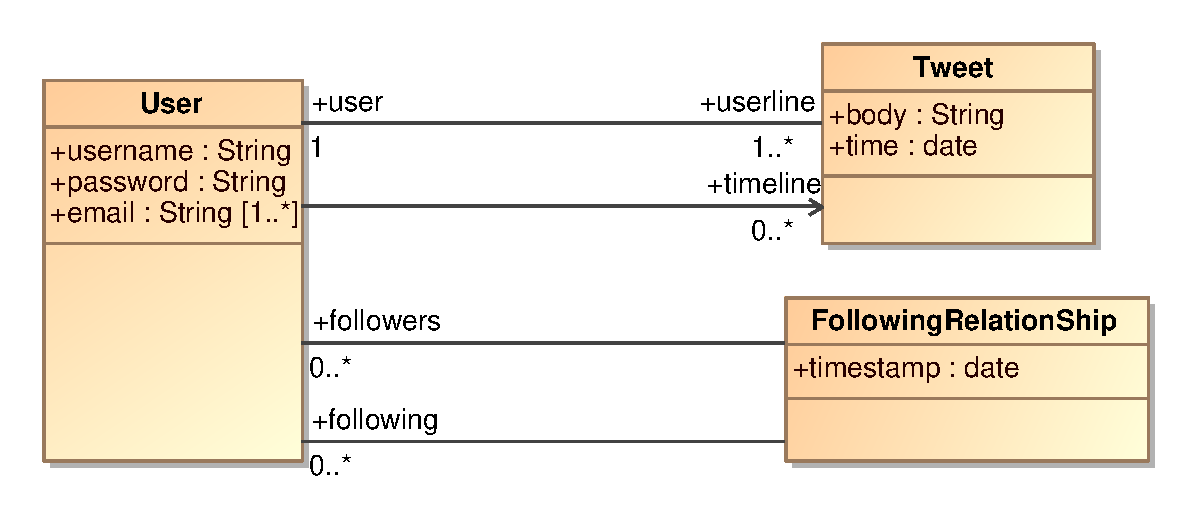
\includegraphics[width=.8\linewidth]{m2m/images/twissandra.eps} \\
  \caption{Modelo UML Twissandra}
  \label{back:fig:twissandra}
\end{figure}

En esta secci�n se presenta el siguiente caso de estudio. Twissandra es un proyecto creado para aprender como utilizar Cassandra. En esta secci�n se reproducir�n los procesos M2M y M2T en el siguiente capitulo, todo esto bajo el proceso de desarrollo dirigido por modelos. El modelo UML correspondiente a Twissandra es el siguiente figura~\ref{back:fig:twissandra}.

Twissandra es una versi�n simplificada de Twitter, que es a menudo utilizada para demostrar las capacidades de Cassandra. Twitter es una red social muy conocida que funciona de la siguiente manera: los usuarios registrados pueden publicar tweets. Un tweet es simplemente un texto con un l�mite de 140 caracteres publicado a una hora determinada. La colecci�n de todos los tweets publicados por un usuario cronol�gicamente ordenados, est�n asignados a su Userline.
Cada usuario registrado en Twissandra puede seguir a otros usuarios registrados. Cuando decimos que Pedro sigue a Mar�a significa que Pedro est� interesado en saber qu� publica Mar�a en su tabl�n. As�, cada usuario registrado tiene tambi�n un timeline que vendr�a a ser la colecci�n de todos los tweets de las personas a las que sigue ordenadas cronol�gicamente.

Los principales casos de uso de un sistema de este tipo son: (1) obtener el timeline de un usuario determinado; (2) obtener el Userline de un usuario, (3) obtener la lista de usuarios que un usuario est� siguiendo; y (4) obtener la lista de usuarios que est�n siguiendo a un usuario espec�fico. Estas dos �ltimas listas deben ser ordenadas cronol�gicamente.

Una vez entendido esto se procede a detallar el proceso de transformaci�n del modelo UML de Twissandra a un modelo que cumpla las restricciones del meta-modelo de Cassandra descrito en la secci�n anterior.

\subsection{Transformaci�n M2M}

Partiendo del modelo UML de la figura~\ref{back:fig:twissandra} y una vez establecidas las reglas de transformaci�n entre modelos, esta secci�n explica el proceso de transformaci�n del modelo UML al modelo Cassandra.

En primer lugar, marcamos el atributo username de la clase User como clave. En el caso de la clase FollowingRelationship y la clase Tweet al no tener un atributo marcado como clave generamos una clave sustituta autom�ticamente para cada clase, llamadas FollowingRelationship\_id y tweet\_id respectivamente.

Por cada paquete estereotipado como <<dataModel>>, se crea un nuevo keyspace. El nombre del keyspace ser� el nombre utilizado por el data model. Los atributos restantes de las meta-clases del keyspace se establecen en sus valores definidos por defecto. A continuaci�n, todos los elementos correspondientes de ese paquete se procesan y se colocan dentro de su keyspace correspondiente.

Como se mencionaba en las reglas de transformaci�n, la clase User se transforma en una Column Family llamada User. A continuaci�n, los atributos y las asociaciones se procesan. Por �ltimo, el atributo Username, que se marc� como clave en el modelo de datos UML, es marcado como Primary Key. De manera similar para aquellos atributos del modelo UML cuya multiplicidad sea igual a uno se realiza una transformaci�n simple, por ejemplo el atributo username y password se transforman en dos columnas, ambos del tipo text. Estas columnas est�n contenidas en la column family User. De la misma manera se transforman los atributos body y time de la clase Tweet y el atributo timestamp de la clase FollowingRelationship.
En el caso de el atributo del modelo UML email cuya multiplicidad es mayor de uno y tiene las propiedades isUnique establecida en true y la propiedad isOrdered establecida en false (en el modelo no se puede apreciar pero esta configurado as�), se transforma este atributo en una list llamada email de tipo text dentro de la column family User.

En cuanto a las asociaciaciones de multiplicidad igual a uno la transformaci�n que se realiza por ejemplo, para la asociaci�n de la clase user una nueva columna llamada user\_username (recordemos que username es la clave de la column family user) es creada y a�adida a la column family Tweet. Para las asociaciones cuya multiplicidad es mayor de uno, por ejemplo la asociaci�n llamada userline se crea una dynamic column family llamada User\_userline. A continuaci�n una columna llamada username de tipo text es a�adida a esta column family. Despu�s una columna llamada tweet\_id de tipo uuid es a�adida (el atributo "tweet\_id" fue creado en la column family tweet al no tener clave). Las columnas user\_username y tweet\_id son designadas como primary key, el atributo user\_username ser� la partition key. 